\Chapter{A játék matematikai modellje}


\begin{figure}[h]
\centering
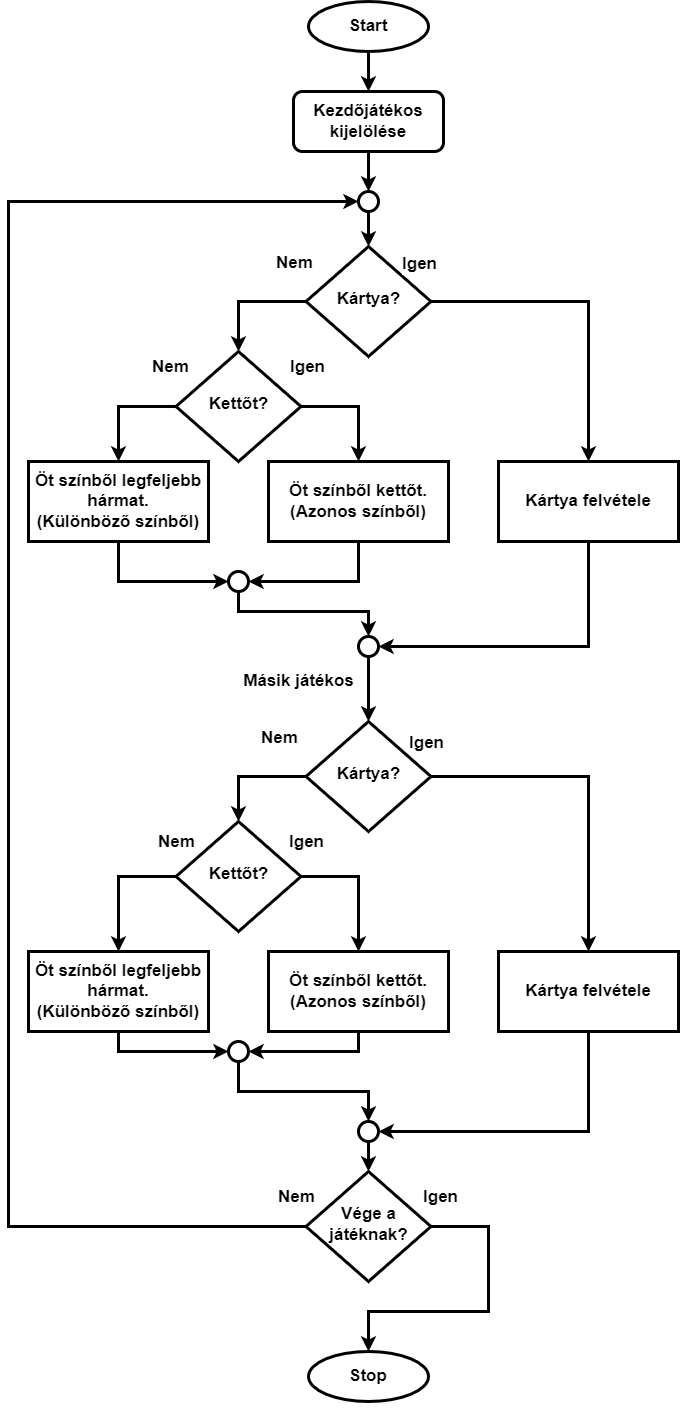
\includegraphics[scale=0.3]{images/flowchart.png}
\caption{A játék folyamatábrája.}
\label{fig:flowchart}
\end{figure}


A játékos természetesen csak a számára elérhető kártyákból és zsetonokból választhat. Egy zseton akkor elérhető a számára, ha abból legalább egy van a játéktéren, a kártya pedig akkor, ha a megvásárlásához szükséges zsetonok a birtokában vannak. Ezek a zsetonok lehetnek sima, korábban elvett zsetonok, vagy akár a kártyák korábbi megvásárlása nyomán megszerzett bónusz értékek.